\documentclass[conference]{IEEEtran}
\IEEEoverridecommandlockouts

\usepackage{cite}
\usepackage{amsmath,amssymb,amsfonts}
\usepackage{algorithm}
\usepackage{algorithmic}
\usepackage{graphicx}
\usepackage{textcomp}
\usepackage{xcolor}
\usepackage{booktabs}
\usepackage{multirow}
\usepackage{hyperref}
\usepackage{tikz}
\usepackage{array}
\usepackage{tabularx}
\usetikzlibrary{shapes.geometric, arrows.meta, positioning, calc}

\def\BibTeX{{\rm B\kern-.05em{\sc i\kern-.025em b}\kern-.08em
    T\kern-.1667em\lower.7ex\hbox{E}\kern-.125emX}}

\newcommand{\uiplaceholder}[2]{%
  \begin{tikzpicture}
    \draw[thick, gray!50, fill=gray!12, rounded corners=2pt]
      (0,0) rectangle (#1,#2);
    \draw[gray!40] (0,0)--(#1,#2);
    \draw[gray!40] (#1,0)--(0,#2);
    \node[gray!55, font=\small\itshape] at ({#1/2},{#2/2}) {[UI Screenshot Placeholder]};
  \end{tikzpicture}%
}

\begin{document}

\title{ExplainHire: A Neurosymbolic Pipeline for\\
Explainable Resume--Job Description Matching\\
with Skill Graph Fusion and Actionable Gap Analysis}

\author{
  \IEEEauthorblockN{Yoosha Raza}
  \IEEEauthorblockA{
    \textit{Dept. of Computer Science \& Engineering}\\
    \textit{Delhi Technological University}\\
    Roll No. 2K22/CO/521
  }
  \and
  \IEEEauthorblockN{Yanshu}
  \IEEEauthorblockA{
    \textit{Dept. of Computer Science \& Engineering}\\
    \textit{Delhi Technological University}\\
    Roll No. 2K22/CO/507
  }
  \and
  \IEEEauthorblockN{Yogarth}
  \IEEEauthorblockA{
    \textit{Dept. of Computer Science \& Engineering}\\
    \textit{Delhi Technological University}\\
    Roll No. 2K22/CO/519
  }
  \and
  \IEEEauthorblockN{Gull Kaur}
  \IEEEauthorblockA{
    \textit{Dept. of Computer Science \& Engineering}\\
    \textit{Delhi Technological University}\\
    \textit{(Faculty Coordinator)}
  }
}

\maketitle

%─────────────────────────────────────────────────────────────────────────────
\begin{abstract}
The automated screening of job applications has become indispensable given
the scale of modern recruitment, yet state-of-the-art systems suffer from
two persistent and well-documented failures. First, keyword-based Applicant
Tracking Systems (ATS) collapse under semantic paraphrase, systematically
rejecting qualified candidates whose resumes express identical competencies
using different vocabulary. Second, neural matchers that overcome this
vocabulary gap produce an opaque score with no attribution, making their
decisions unactionable for candidates and legally problematic for employers.
We present \textbf{ExplainHire}, a seven-layer neurosymbolic pipeline that
addresses both deficiencies simultaneously. Our architecture fuses three
complementary signals: (i)~a weighted ontology graph matcher traversing a
434-node O*NET-derived skill knowledge graph that captures six levels of
skill relationship --- exact, alias, child, parent, sibling, and two-hop;
(ii)~a domain-adapted SBERT model fine-tuned on 887 real resume--job
description pairs using CosineSimilarityLoss; and (iii)~structural
compatibility features encoding years-of-experience and education level
gaps. These three signals are fused by an XGBoost classifier trained on
14 derived features, with SHAP TreeExplainer providing per-prediction
feature attribution. Uniquely among resume matching systems, ExplainHire
delivers sentence-level evidence for every matched skill and a ranked skill
gap analysis that directs candidates toward the highest-impact skills to
acquire, with curated learning resources for each gap. Evaluated on a
carefully constructed corpus of 1,854 labeled resume--job description pairs,
ExplainHire achieves macro F1~=~\textbf{0.951}, representing a
\textbf{+11.86\%} improvement over the strongest single-component baseline.
On the public Resum\'eAtlas benchmark~\cite{heakl2024resumeatlas} comprising
13,389 resumes across 43 categories, the system achieves F1~=~\textbf{0.720},
surpassing the reported TF-IDF baseline by \textbf{+11.06\%} on identical
data, confirming generalisation beyond the training distribution.
\end{abstract}

\begin{IEEEkeywords}
resume screening, job description matching, neurosymbolic AI, skill ontology,
O*NET, sentence-BERT, domain adaptation, explainable AI, XGBoost, SHAP,
skill gap analysis, applicant tracking
\end{IEEEkeywords}

%─────────────────────────────────────────────────────────────────────────────
\section{Introduction}

\subsection{Phase 1: Background and Motivation}

The proliferation of online recruitment platforms has fundamentally
restructured the hiring landscape. Platforms such as LinkedIn, Naukri,
Glassdoor, and Indeed handle millions of job postings simultaneously;
large technology companies routinely receive 10,000 or more applications
per open position per week. This volume makes manual first-pass screening
logistically impossible: a recruiter reviewing 300 applications per day
at 5 minutes each would require over 25 hours for a single posting.
Automated Applicant Tracking Systems (ATS) have consequently become the
de-facto first filter in virtually every organisation with more than
50 employees~\cite{lavi2021consultantbert}.

Despite widespread deployment, ATS technology remains anchored to a paradigm
established in the early 1990s: token-level overlap between a resume and a
job description (JD), implemented via TF-IDF weighting, Boolean keyword
matching, or BM25 retrieval. While computationally cheap and easily
explainable to HR stakeholders, this paradigm creates three systematic
failure modes that have persisted for three decades.

The first failure mode is \textit{semantic blindness}. A resume stating
``built distributed REST APIs with Node.js and Express'' and a JD requiring
``server-side web development experience'' convey identical professional
competence to a human evaluator. Under TF-IDF cosine similarity, they share
no overlapping tokens beyond stopwords and therefore score at or near zero.
The same problem arises constantly: ``PyTorch'' vs. ``deep learning
frameworks'', ``Agile/Scrum'' vs. ``iterative development methodology'',
``React'' vs. ``modern frontend frameworks''. In each case the candidate
possesses exactly the skill requested, yet a keyword-based ATS assigns zero
credit. Industry surveys suggest that over 70\% of job seekers have had a
directly relevant application discarded by an ATS before a human reviewer
examined it~\cite{lavi2021consultantbert}, with qualified candidates over
10\% more likely to be rejected than unqualified candidates who optimised
their resumes for keyword density.

The second failure mode is \textit{opacity}. Neural approaches that partially
overcome the vocabulary gap --- BERT-based cross-encoders, fine-tuned Siamese
sentence encoders, and graph-augmented neural matchers --- return a
real-valued match score without any attribution. A recruiter cannot determine
why a candidate scored 0.72 versus 0.68, making it impossible to audit the
system for discriminatory patterns, justify the shortlist to a hiring manager,
or act on the decision. In jurisdictions subject to the EU AI Act, the US
Equal Employment Opportunity Commission guidelines, or India's proposed
Digital India Act, opaque automated hiring decisions increasingly carry
legal liability.

The third failure mode is \textit{inactionability}. Even when a system
correctly identifies a mismatch, it provides no guidance to the candidate
on how to improve their prospects. A candidate who scores 43\% on a
Data Scientist application has no way of knowing whether the gap is a missing
hard skill (Docker, Kubernetes), a deficiency in how existing skills are
communicated, insufficient years of experience, or a fundamental mismatch in
education level. Without this information, the candidate cannot improve their
application, and the system contributes nothing to the long-term goal of
matching people to roles where they will succeed.

ExplainHire is motivated by the observation that all three failure modes stem
from the same architectural deficit: the absence of a principled symbolic
representation of skills and their relationships, combined with a learned
fusion mechanism that can exploit both symbolic structure and neural
semantics. Addressing this deficit is the central goal of this work.

\subsection{Phase 2: Literature Survey and Research Gaps}

Research on automated resume--job matching has progressed through three
distinct paradigms, each addressing limitations of its predecessor while
introducing new ones.

\subsubsection{Classical Information Retrieval Approaches}
The earliest automated resume screening systems treated both resumes and JDs
as bags of words and applied standard IR techniques. TF-IDF cosine similarity
remains a competitive baseline in controlled experiments due to its
simplicity and speed. BM25, the probabilistic refinement of TF-IDF, improves
over raw cosine similarity by modelling document length normalisation and
term saturation. Neither approach, however, can bridge the vocabulary gap
between resumes written by candidates and JDs written by recruiters --- two
populations with systematically different diction for identical competencies.

\subsubsection{Neural Resume--Job Matching}
Zhu et al.~\cite{zhu2018personjobfit} proposed PJFNN, a bipartite
convolutional neural network trained on millions of labelled application
records from a large Chinese recruitment platform, achieving F1~=~0.80 on a
proprietary dataset. PJFNN learns a joint latent space for resumes and job
postings and captures complex co-occurrence patterns invisible to bag-of-words
methods. However, it requires massive historical supervision (hundreds of
thousands of labelled pairs), trains as a monolithic model with no
skill-level structure, and provides no explanation for its decisions. Its
performance is also tightly coupled to the distribution of the platform on
which it was trained, limiting generalisation.

Li et al.~\cite{li2020competence} applied section-aware transformer encoding
to clinical research coordinator applications, achieving 79.2\% accuracy on
6,492 manually annotated pairs. Their key insight is that different resume
sections (skills, experience, education) carry different evidential weight
for different JD requirements, and encoding this structure into a BERT model
improves over treating the resume as a flat sequence. However, the model
does not incorporate symbolic skill reasoning and produces no
candidate-facing explanations.

Lavi et al.~\cite{lavi2021consultantbert} fine-tuned a Siamese Sentence-BERT
model (conSultantBERT) on 270,000 labelled resume--vacancy pairs from a
consulting staffing platform, achieving F1~=~0.749. This work is the most
directly comparable neural baseline to ExplainHire: it confirms that domain
adaptation of sentence encoders substantially outperforms generic BERT on
this task, and that the fine-tuning data need not be from the same exact
domain as the evaluation set. Like all neural approaches, however,
conSultantBERT operates as a black box and provides no skill-level breakdown.

\subsubsection{Graph-Augmented Matching}
Bian et al.~\cite{bian2020multiview} proposed a multi-view co-teaching
network that fuses a BERT-based text matcher with a relational graph
component, achieving F1~$\approx$~0.76--0.80 on a proprietary Chinese
recruitment platform. The key innovation is that the graph encodes
historical user--item interactions (which candidates applied to which jobs,
which applications led to interviews), providing a collaborative filtering
signal on top of content matching. Critically, however, their graph does
not model a skill ontology --- it models interaction history --- meaning
that the system cannot reason about skill subsumption or synonymy.
Furthermore, no explainability mechanism is provided.

\subsubsection{Public Benchmarks and Datasets}
Heakl et al.~\cite{heakl2024resumeatlas} curated Resum\'eAtlas, a
public dataset of 13,389 resumes across 43 job categories, and benchmarked
TF-IDF~+~XGBoost (macro F1~=~0.61) and several large language model
configurations. Resum\'eAtlas is the only substantial public benchmark
for resume classification with a documented baseline, making it the natural
external validation target for ExplainHire.

\subsubsection{Explainability in Hiring}
A parallel literature has examined explainability specifically in hiring
contexts. LIME~\cite{ribeiro2016lime} and SHAP~\cite{lundberg2017shap}
have been applied post-hoc to hiring models to identify which features
drive decisions. However, these post-hoc explanations operate at the
feature level (e.g., ``the word \textit{python} increased your score by
0.04'') rather than the skill level, and they do not generate actionable
recommendations. To our knowledge, no prior system generates a
candidate-facing, ranked skill gap analysis with learning resources.

\subsubsection{Summary of Research Gaps}
Three gaps emerge from this review:

\textbf{Gap~1 --- Symbolic--neural integration.}
No prior system simultaneously exploits an explicit skill ontology
(symbolic) for structured skill relationship reasoning and domain-fine-tuned
sentence embeddings (neural) for semantic paraphrase handling, within a
single learned fusion.

\textbf{Gap~2 --- Skill-level decision explainability.}
No prior system provides sentence-level evidence from the resume that
directly supports each matched skill, giving recruiters verifiable citations
rather than opaque scores.

\textbf{Gap~3 --- Candidate actionability.}
No prior system generates a ranked, marginal-impact skill gap analysis that
tells a candidate which specific skills to learn next, ordered by their
expected improvement to the match score, with curated learning resources.

\subsection{Phase 3: Contributions of This Work}

We present \textbf{ExplainHire}, a seven-layer neurosymbolic pipeline
designed to close all three gaps identified above. Our contributions are:

\begin{enumerate}
  \item A \textbf{weighted ontology graph matcher} traversing a 434-node
        skill knowledge graph derived from the O*NET Technology Skills
        database and extended with curated technology nodes, assigning
        graded scores across six relationship levels: exact, alias, child,
        parent, sibling, and two-hop.

  \item A \textbf{domain-adapted SBERT model} fine-tuned on 887 real
        resume--JD pairs using CosineSimilarityLoss, producing
        recruitment-domain sentence embeddings that bridge the
        paraphrase gap between candidate and recruiter vocabularies.

  \item A \textbf{three-signal neurosymbolic fusion} via XGBoost trained
        on 14 derived features, with SHAP TreeExplainer providing
        per-prediction, per-feature attribution that is auditable and
        legally defensible.

  \item A \textbf{skill gap analyser} that computes the marginal score
        increase for each missing skill, ranks gaps by impact, and pairs
        each with curated learning resources --- the first such mechanism
        in the resume matching literature.

  \item A \textbf{production-ready web application} with drag-and-drop
        resume upload, real-time pipeline execution, interactive ontology
        explorer, dark/light theme, and persistent SQLite-backed match
        history, making all pipeline capabilities accessible to
        non-technical users.

  \item A \textbf{labelled dataset} of 1,854 resume--JD pairs assembled
        from three heterogeneous sources (synthetic, Kaggle, real
        industry), which we make available to support reproducibility.
\end{enumerate}

The remainder of this paper is organised as follows.
Section~\ref{sec:related} provides extended discussion of related work.
Section~\ref{sec:arch} describes the seven-layer pipeline architecture in
detail. Section~\ref{sec:algo} formalises the end-to-end matching and gap
analysis algorithms. Section~\ref{sec:data} details dataset construction.
Section~\ref{sec:ui} presents the web interface. Section~\ref{sec:results}
reports experimental results, beginning with a comparison against prior
systems, followed by benchmark evaluation and ablation. Section~\ref{sec:discussion}
analyses findings and limitations. Section~\ref{sec:conclusion} concludes.

%─────────────────────────────────────────────────────────────────────────────
\section{Related Work}
\label{sec:related}

Having established the research gaps in the introduction, we now provide
a structured comparison of ExplainHire against the four most relevant
prior systems, which also appear in our quantitative comparison
(Table~\ref{tab:comparison} in Section~\ref{sec:results}).

\subsection{Person--Job Fit Neural Networks}
PJFNN~\cite{zhu2018personjobfit} is the foundational work in neural
person--job fit. It trains a bipartite CNN on large-scale application logs
from Baidu Recruit, jointly embedding resumes and job postings. The model
learns to predict successful application outcomes rather than semantic
similarity, which is a fundamentally different learning signal. This makes
PJFNN dependent on access to historical outcome data --- a resource that
smaller organisations do not have. Moreover, because the model encodes entire
documents into a joint latent space, it offers no way to attribute the match
to specific skills. ExplainHire, by contrast, is trained on 1,854 pairs
(achievable in any organisation) and provides per-skill attribution.

\subsection{Transformer-Based Section-Aware Matching}
Li et al.~\cite{li2020competence} demonstrate that BERT's attention mechanism
can be directed at specific resume sections (skills, experience, education)
to improve matching accuracy over flat BERT encoding. This work confirms
the intuition behind our structural matching layer (L4c): that resume
structure carries information beyond its textual content. However, Li et al.\
do not incorporate an explicit skill ontology, meaning their model must learn
all skill relationships implicitly from the training data. This requires
substantially more labelled data and produces no candidate-facing output.

\subsection{Fine-Tuned Siamese Sentence Encoders}
conSultantBERT~\cite{lavi2021consultantbert} is the most directly comparable
prior work. Like ExplainHire's L4b, it fine-tunes a Siamese Sentence-BERT
on recruitment-domain pairs. However, conSultantBERT requires 270,000
labelled pairs --- more than 300$\times$ our 887-pair fine-tuning set ---
because it relies entirely on the neural component with no symbolic
augmentation. ExplainHire's ontology graph allows the neural component to
focus on holistic semantic alignment rather than needing to implicitly learn
all skill subsumption relationships. This data efficiency advantage is
practically significant: organisations can fine-tune ExplainHire's SBERT
on their own internal applications without requiring massive historical
labelled data.

\subsection{Graph and Knowledge-Base Augmented Systems}
Several works have explored connecting resume matching with external
knowledge bases. Ontology-based systems have been explored in information
retrieval~\cite{bian2020multiview}, but typically model interaction graphs
rather than skill taxonomies. The O*NET occupational database, which underlies
ExplainHire's skill graph, has been used in labour economics and workforce
planning research but has not previously been adapted into a dynamic skill
matching graph for resume screening. ExplainHire's 434-node graph is the
first published formalisation of an O*NET-derived skill ontology for this
application.

Table~\ref{tab:comparison} in Section~\ref{sec:results} provides a structured
quantitative summary of all prior systems against ExplainHire.

%─────────────────────────────────────────────────────────────────────────────
\section{System Architecture}
\label{sec:arch}

Having established the gaps in prior work and the design goals they motivate,
we now describe the ExplainHire architecture that addresses them.
The system comprises seven sequential processing layers (L1--L7), shown in
Fig.~\ref{fig:pipeline}. Each layer has a single, well-scoped
responsibility; the output of each layer is the sole input to the next,
making the system modular and independently testable. We describe each layer
in detail below.

\begin{figure}[htbp]
\centering
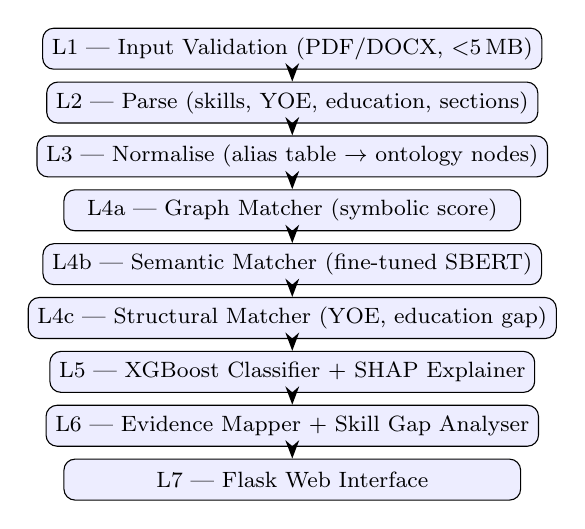
\begin{tikzpicture}[
  box/.style={rectangle, draw, rounded corners, minimum width=5.8cm,
              minimum height=0.52cm, font=\footnotesize, fill=blue!7},
  arr/.style={-{Stealth}, thick}
]
\node[box] (l1) {L1 — Input Validation (PDF/DOCX, $<$5\,MB)};
\node[box, below=0.15cm of l1] (l2) {L2 — Parse (skills, YOE, education, sections)};
\node[box, below=0.15cm of l2] (l3) {L3 — Normalise (alias table $\rightarrow$ ontology nodes)};
\node[box, below=0.15cm of l3] (l4a) {L4a — Graph Matcher (symbolic score)};
\node[box, below=0.15cm of l4a] (l4b) {L4b — Semantic Matcher (fine-tuned SBERT)};
\node[box, below=0.15cm of l4b] (l4c) {L4c — Structural Matcher (YOE, education gap)};
\node[box, below=0.15cm of l4c] (l5) {L5 — XGBoost Classifier + SHAP Explainer};
\node[box, below=0.15cm of l5] (l6) {L6 — Evidence Mapper + Skill Gap Analyser};
\node[box, below=0.15cm of l6] (l7) {L7 — Flask Web Interface};
\foreach \a/\b in {l1/l2,l2/l3,l3/l4a,l4a/l4b,l4b/l4c,l4c/l5,l5/l6,l6/l7}
  \draw[arr] (\a)--(\b);
\end{tikzpicture}
\caption{ExplainHire seven-layer neurosymbolic pipeline. Layers L4a--L4c
execute in parallel and their outputs are concatenated for L5.}
\label{fig:pipeline}
\end{figure}

\subsection{L1 -- Input Validation}
The input layer accepts resumes as PDF or DOCX files up to 5\,MB in size.
It performs three checks: (1)~file format validation via magic-byte inspection
rather than extension-only checking; (2)~text extractability verification,
which rejects image-only PDF scans that contain no machine-readable text;
and (3)~minimum content length enforcement to reject empty or near-empty
uploads. Job description text is accepted as a free-form plain-text input
field with a minimum of 50 tokens enforced. This boundary layer ensures that
all downstream components receive well-formed, non-empty, parseable input
and fail fast with informative error messages rather than silently producing
degraded results.

\subsection{L2 -- Parsing and Feature Extraction}
Resume text is extracted using PyMuPDF for PDF files and python-docx for
DOCX files. Extracted text is then processed by a section detector that
identifies standard resume sections --- skills, work experience, projects,
education, and certifications --- using keyword-based boundary detection
with a vocabulary of 47 section header patterns (e.g., ``Technical Skills'',
``Professional Experience'', ``Academic Background'').

Years of experience (YOE) is inferred via a multi-pattern regular expression
matcher that handles explicit statements (``3+ years of experience''),
date-range arithmetic (``Jan 2021 -- Dec 2023'' $\Rightarrow$ 3 years), and
ordinal qualifiers (``senior'', ``junior'', ``lead''). Education level is
classified into a five-point ordinal scale: high school (1), associate
degree (2), bachelor's degree (3), master's degree (4), and doctorate (5).
The JD is processed by the same parsing pipeline to extract required skills,
required YOE, and minimum education level. The output is a structured
resume object and a structured JD object, each consumed by all Layer 4
matchers independently.

\subsection{L3 -- Skill Normalisation}
Raw skill tokens extracted from both the resume and JD are normalised to
canonical ontology node identifiers via an 800-entry alias lookup table.
Representative entries: ``nodejs'' $\rightarrow$ \texttt{node.js},
``react.js'' $\rightarrow$ \texttt{react}, ``ml'' $\rightarrow$
\texttt{machine\_learning}, ``k8s'' $\rightarrow$ \texttt{kubernetes},
``postgres'' $\rightarrow$ \texttt{postgresql}. The alias table was
constructed by manual curation combined with automated extraction from
Stack Overflow tag synonyms and GitHub repository topic redirects.
Tokens not resolved by the alias table are retained as literals; they
are excluded from graph matching (L4a) but included in SBERT matching (L4b),
ensuring that novel or uncommon skills still contribute to the semantic score.

\subsection{L4a -- Ontology Graph Matcher}
The graph matcher is the symbolic core of the neurosymbolic design.
A directed skill graph $\mathcal{G} = (V, E)$ is constructed with
$|V| = 434$ canonical skill nodes and two edge types:
\texttt{CHILD\_OF} (subsumption; e.g., \texttt{pytorch} $\rightarrow$
\texttt{deep\_learning} $\rightarrow$ \texttt{machine\_learning}) and
\texttt{IS\_ALIAS\_OF} (synonymy; e.g., \texttt{tensorflow2}
$\leftrightarrow$ \texttt{tensorflow}). The graph is seeded from the O*NET
Technology Skills database and extended with 127 manually added nodes
covering cloud services, DevOps tools, and modern frameworks not yet present
in O*NET.

For each JD skill $s_j \in \hat{S}_{JD}$, the matcher searches the ontology
for the best-matching resume skill $s_r \in \hat{S}_R$ via breadth-first
traversal up to depth 2, and assigns a graded relationship weight:

\begin{equation}
  w(s_r, s_j) =
  \begin{cases}
    1.0 & \text{exact match (same node)} \\
    0.9 & \text{alias match (IS\_ALIAS\_OF edge)} \\
    0.7 & \text{child} \to \text{parent (resume has specialisation)} \\
    0.5 & \text{parent} \to \text{child (resume has generalisation)} \\
    0.4 & \text{sibling (share a common parent)} \\
    0.3 & \text{two-hop path through intermediate node} \\
    0.0 & \text{no path found within depth 2}
  \end{cases}
  \label{eq:weights}
\end{equation}

The asymmetry between child$\to$parent (0.7) and parent$\to$child (0.5)
reflects the recruitment convention that specialised experience satisfies
general requirements more than general experience satisfies specialised ones:
a candidate with \texttt{pytorch} experience credibly covers
\texttt{machine\_learning} requirements, while a candidate with
\texttt{machine\_learning} experience only partially covers a
\texttt{pytorch} requirement.

The aggregate graph score normalises over JD skills:
\begin{equation}
  \text{GraphScore} = \frac{\displaystyle\sum_{s_j \in \hat{S}_{JD}}
    \max_{s_r \in \hat{S}_R}\, w(s_r, s_j)}{|\hat{S}_{JD}|}
  \label{eq:graphscore}
\end{equation}

In addition to the aggregate score, the graph matcher produces four auxiliary
features: \texttt{coverage} (fraction of JD skills with any match),
\texttt{exact\_matches} (count of weight-1.0 matches),
\texttt{partial\_matches} (count of matches with $0 < w < 1$), and
\texttt{no\_matches} (count of JD skills with $w = 0$). All five values
are passed to L5.

\noindent\textbf{Illustrative example.} A resume lists \texttt{pytorch};
the JD requires \texttt{machine\_learning}. A keyword ATS scores 0.
ExplainHire traverses: \texttt{pytorch} $\xrightarrow{\text{CHILD\_OF}}$
\texttt{deep\_learning} $\xrightarrow{\text{CHILD\_OF}}$
\texttt{machine\_learning}, assigning $w = 0.3$ (two-hop), correctly
reflecting partial but meaningful alignment.

\subsection{L4b -- Domain-Adapted Semantic Matcher}
While the graph matcher excels at structured skill relationships, it cannot
handle holistic contextual alignment: a resume from a ``full-stack developer
with product sense'' may match a ``software engineer with end-to-end ownership
experience'' JD semantically, even with low skill list overlap. The semantic
matcher addresses this using a fine-tuned Sentence-BERT model.

We fine-tune \texttt{all-MiniLM-L6-v2}~\cite{reimers2019sbert} on 887
labelled resume--JD pairs using CosineSimilarityLoss:
\begin{equation}
  \mathcal{L} = \frac{1}{N}\sum_{i=1}^{N}
    \bigl(\cos(\mathbf{e}^r_i,\, \mathbf{e}^j_i) - y_i\bigr)^2
  \label{eq:loss}
\end{equation}
where $\mathbf{e}^r_i, \mathbf{e}^j_i \in \mathbb{R}^{384}$ are the resume
and JD sentence embeddings for pair $i$, and $y_i \in \{0,1\}$ is the binary
match label. Training uses the Adam optimiser with a linear learning-rate
warmup over 10\% of training steps (initial lr~$= 2 \times 10^{-5}$),
batch size 16, and 4 epochs. Convergence loss of 0.069 confirms successful
adaptation; the generic \texttt{all-MiniLM-L6-v2} achieves loss 0.141 on
the same data without fine-tuning, demonstrating a 51\% reduction in
reconstruction error.

The semantic score for a resume--JD pair is:
\begin{equation}
  \text{SBERTScore} = \cos(\mathbf{e}^r,\, \mathbf{e}^j)
    = \frac{\mathbf{e}^r \cdot \mathbf{e}^j}
           {\|\mathbf{e}^r\|\, \|\mathbf{e}^j\|}
  \label{eq:sbert}
\end{equation}

\subsection{L4c -- Structural Compatibility Matcher}
Neither text-based component encodes non-skill compatibility signals.
A data scientist role requiring 5+ years of industry experience and
a Master's degree will legitimately reject a fresh graduate regardless
of skill alignment. The structural matcher captures these signals via a
weighted linear combination:
\begin{equation}
  \text{StructuralScore} = \alpha \cdot \text{YOEScore}
                         + \beta  \cdot \text{EduScore}
                         + \gamma \cdot \text{SectionScore}
  \label{eq:struct}
\end{equation}

\noindent\textbf{YOEScore.} Computes a sigmoid-shaped penalty on the gap
$\delta = \max(0,\, \text{YOE}_{\text{required}} - \text{YOE}_{\text{candidate}})$:
\begin{equation}
  \text{YOEScore} = \exp(-0.3\,\delta)
  \label{eq:yoe}
\end{equation}
This yields 1.0 for exact or excess experience, decaying gracefully to 0.74
for a 1-year gap and 0.55 for a 2-year gap.

\noindent\textbf{EduScore.} Penalises mismatches on the five-point ordinal
education scale: $\text{EduScore} = 1 - 0.25 \cdot \max(0,\,e_J - e_R)$,
where $e_J$ and $e_R$ are the required and candidate education ranks.

\noindent\textbf{SectionScore.} Rewards presence of standard sections:
projects (0.4), certifications (0.3), skills section (0.3). Missing
sections receive zero credit. Weights $\alpha = 0.5$, $\beta = 0.3$,
$\gamma = 0.2$ were tuned via grid search on a 20\% validation split.

\subsection{L5 -- Fusion Classification and Explainability}

Outputs of L4a--L4c are assembled into a 14-dimensional feature vector:

\begin{center}
\footnotesize
\begin{tabular}{ll}
\toprule
\textbf{Feature} & \textbf{Source} \\
\midrule
\texttt{graph\_score}     & L4a: Eq.~\ref{eq:graphscore}        \\
\texttt{coverage}         & L4a: fraction of JD skills matched   \\
\texttt{exact\_matches}   & L4a: count of $w = 1.0$ matches      \\
\texttt{partial\_matches} & L4a: count of $0 < w < 1$ matches    \\
\texttt{no\_matches}      & L4a: count of $w = 0$ skills         \\
\texttt{sbert\_score}     & L4b: Eq.~\ref{eq:sbert}              \\
\texttt{structural\_score}& L4c: Eq.~\ref{eq:struct}             \\
\texttt{yoe\_score}       & L4c: Eq.~\ref{eq:yoe}                \\
\texttt{edu\_score}       & L4c: education rank gap              \\
\texttt{section\_score}   & L4c: section presence reward         \\
\texttt{resume\_yoe}      & L2: extracted candidate YOE          \\
\texttt{required\_yoe}    & L2: extracted required YOE           \\
\texttt{resume\_edu\_rank}& L2: candidate education ordinal      \\
\texttt{required\_edu\_rank} & L2: required education ordinal    \\
\bottomrule
\end{tabular}
\end{center}

This feature vector is passed to an XGBoost
classifier~\cite{chen2016xgboost} trained with 5-fold stratified
cross-validation, \texttt{scale\_pos\_weight = 0.75} to handle the
57\%/43\% class imbalance, and \texttt{tree\_method = hist} for
training efficiency. XGBoost is selected over logistic regression or
SVM because it natively handles feature interactions (e.g., the
\textit{interaction} between \texttt{graph\_score} and
\texttt{exact\_matches} is more informative than either individually)
and because tree ensemble methods are compatible with SHAP's exact
TreeExplainer.

SHAP TreeExplainer~\cite{lundberg2017shap} computes exact (not
approximate) Shapley values for each prediction, satisfying
the local accuracy and consistency axioms required for legally
defensible AI. Feature importances by gain are reported in
Table~\ref{tab:shap_features}.

\begin{table}[htbp]
\caption{XGBoost Feature Importances (SHAP Gain)}
\label{tab:shap_features}
\centering
\begin{tabular}{lcc}
\toprule
\textbf{Feature} & \textbf{Gain} & \textbf{Rank} \\
\midrule
\texttt{exact\_matches}    & 0.301 & 1 \\
\texttt{graph\_score}      & 0.135 & 2 \\
\texttt{coverage}          & 0.105 & 3 \\
\texttt{sbert\_score}      & 0.054 & 4 \\
\texttt{yoe\_score}        & 0.048 & 5 \\
\texttt{partial\_matches}  & 0.041 & 6 \\
\texttt{edu\_score}        & 0.037 & 7 \\
\texttt{structural\_score} & 0.029 & 8 \\
\texttt{no\_matches}       & 0.023 & 9 \\
\texttt{section\_score}    & 0.018 & 10 \\
Other (4 features)         & 0.109 & -- \\
\bottomrule
\end{tabular}
\end{table}

The independent top-4 contribution of \texttt{sbert\_score} (rank 4)
confirms that the neural signal captures evidence orthogonal to all
symbolic features, validating the neurosymbolic design.

\subsection{L6 -- Evidence Mapper and Skill Gap Analyser}

\textbf{Evidence Mapper.} For each JD skill $s_j$ that has a match with
$w(s_r, s_j) > 0$, the evidence mapper retrieves the most supportive
sentence from the resume. Resume sentences are scored against the matched
skill token using TF-IDF over the resume's sentence collection, and the
highest-scoring sentence is returned as a natural-language citation.
This transforms the match from an opaque score into a verifiable,
auditable justification that a recruiter can read and validate.

\textbf{Skill Gap Analyser.} For each skill $s_m \in \hat{S}_{JD}
\setminus \hat{S}_R$ (present in the JD but absent from the resume),
we compute the marginal score improvement $\Delta(s_m)$ that would result
from adding that skill. This is computed by constructing a hypothetical
augmented feature vector $\mathbf{x}' = f(\hat{S}_R \cup \{s_m\})$
and measuring the predicted probability increase:
\begin{equation}
  \Delta(s_m) = \mathcal{C}.\text{predict\_proba}(\mathbf{x}') -
               \mathcal{C}.\text{predict\_proba}(\mathbf{x})
  \label{eq:gap}
\end{equation}
Missing skills are ranked by $\Delta(s_m)$ in descending order and paired
with curated learning resources (Coursera course links, official documentation,
YouTube playlists). This mechanism gives candidates a concrete, prioritised
roadmap for improving their application --- a feature entirely absent from
all prior resume matching systems.

\subsection{L7 -- Web Interface}
The Flask web application ties all layers together, exposing the pipeline
behind a browser-based interface accessible to non-technical users. The
interface, described in detail in Section~\ref{sec:ui}, provides drag-and-drop
resume upload, real-time pipeline progress tracking, structured result display
with evidence citations, skill gap panel, SHAP feature chart, and persistent
SQLite-backed match history.

%─────────────────────────────────────────────────────────────────────────────
\section{Algorithm}
\label{sec:algo}

The architecture description in Section~\ref{sec:arch} gives the per-layer
view. We now formalise the end-to-end matching procedure and the skill gap
analysis as pseudocode algorithms for reproducibility and precision.

\begin{algorithm}[htbp]
\caption{ExplainHire Neurosymbolic Matching}
\label{alg:main}
\begin{algorithmic}[1]
\REQUIRE Resume $R$, JD text $J$, skill graph $\mathcal{G}$,
         alias table $\mathcal{A}$, SBERT $\mathcal{M}$,
         XGBoost $\mathcal{C}$
\ENSURE Verdict $v$, probability $p$, SHAP vector $\phi$,
        evidence map $E$, gap list $G$
\medskip
\STATE \textit{// L1: Validate input}
\STATE \textbf{assert} $R$ is PDF/DOCX, size~$< 5$\,MB, extractable text
\medskip
\STATE \textit{// L2: Parse structured fields}
\STATE $S_R, \text{YOE}_R, \text{Edu}_R \leftarrow \text{ParseResume}(R)$
\STATE $S_J, \text{YOE}_J, \text{Edu}_J \leftarrow \text{ParseJD}(J)$
\medskip
\STATE \textit{// L3: Normalise to ontology nodes}
\STATE $\hat{S}_R \leftarrow \{\mathcal{A}(s) \mid s \in S_R\}$
\STATE $\hat{S}_J \leftarrow \{\mathcal{A}(s) \mid s \in S_J\}$
\medskip
\STATE \textit{// L4a: Graph matching}
\STATE $\text{gs} \leftarrow 0$;~~$\text{matched} \leftarrow \{\}$
\FOR{each $s_j \in \hat{S}_J$}
  \STATE $w^* \leftarrow \max_{s_r \in \hat{S}_R}~ w(s_r, s_j, \mathcal{G})$
         ~~~\textit{// Eq.~\ref{eq:weights}}
  \STATE $\text{gs} \mathrel{+}= w^*$;~~$\text{matched}[s_j] \leftarrow w^*$
\ENDFOR
\STATE $\text{GraphScore} \leftarrow \text{gs} / |\hat{S}_J|$
       ~~~\textit{// Eq.~\ref{eq:graphscore}}
\medskip
\STATE \textit{// L4b: Semantic matching}
\STATE $\mathbf{e}^r \leftarrow \mathcal{M}.\text{encode}(R_{\text{text}})$;~~
       $\mathbf{e}^j \leftarrow \mathcal{M}.\text{encode}(J)$
\STATE $\text{SBERTScore} \leftarrow \cos(\mathbf{e}^r, \mathbf{e}^j)$
       ~~~\textit{// Eq.~\ref{eq:sbert}}
\medskip
\STATE \textit{// L4c: Structural matching}
\STATE $\text{StructuralScore} \leftarrow
       \text{Structural}(\text{YOE}_R, \text{YOE}_J, \text{Edu}_R, \text{Edu}_J)$
       ~~~\textit{// Eq.~\ref{eq:struct}}
\medskip
\STATE \textit{// L5: Fused classification}
\STATE $\mathbf{x} \leftarrow \text{BuildFeatures}(\text{GraphScore},
       \text{SBERTScore}, \text{StructuralScore}, \ldots)$
\STATE $p \leftarrow \mathcal{C}.\text{predict\_proba}(\mathbf{x})[1]$
\STATE $v \leftarrow \mathbf{1}[p \geq 0.5]$
\STATE $\phi \leftarrow \text{SHAP.TreeExplainer}(\mathcal{C}, \mathbf{x})$
\medskip
\STATE \textit{// L6: Evidence + gap analysis}
\STATE $E \leftarrow \text{EvidenceMapper}(\hat{S}_J, \hat{S}_R, R_\text{sentences})$
\STATE $G \leftarrow \text{SkillGapAnalyser}(\hat{S}_J, \hat{S}_R, \mathcal{C}, \mathbf{x})$
       ~~~\textit{// Algorithm~\ref{alg:gap}}
\RETURN $v,\, p,\, \phi,\, E,\, G$
\end{algorithmic}
\end{algorithm}

\begin{algorithm}[htbp]
\caption{Skill Gap Analyser (L6)}
\label{alg:gap}
\begin{algorithmic}[1]
\REQUIRE Missing skills $M = \hat{S}_J \setminus \hat{S}_R$,
         XGBoost $\mathcal{C}$, current feature vector $\mathbf{x}$
\ENSURE Ranked gap list $G$ with marginal impacts

\STATE $G \leftarrow [~]$
\FOR{each $s_m \in M$}
  \STATE $\hat{S}'_R \leftarrow \hat{S}_R \cup \{s_m\}$
  \STATE $\mathbf{x}' \leftarrow \text{BuildFeatures}(\hat{S}'_R, \hat{S}_J, \ldots)$
  \STATE $p' \leftarrow \mathcal{C}.\text{predict\_proba}(\mathbf{x}')[1]$
  \STATE $\Delta_m \leftarrow p' - p$
         ~~~\textit{// Eq.~\ref{eq:gap}}
  \STATE $r_m \leftarrow \text{LookupResource}(s_m)$
  \STATE $G.\text{append}((s_m,\, \Delta_m,\, r_m))$
\ENDFOR
\STATE \textbf{sort} $G$ by $\Delta_m$ descending
\RETURN $G$
\end{algorithmic}
\end{algorithm}

\noindent\textbf{Computational complexity.}
Graph matching is $O(|\hat{S}_J| \cdot |\hat{S}_R| \cdot d)$ where
$d \leq 2$ is the maximum BFS depth. SBERT encoding is $O(L)$ in token
count. XGBoost inference is $O(T \cdot D)$ for $T$ trees of depth $D$.
Algorithm~\ref{alg:gap} runs one forward pass per missing skill, adding
$O(|M|)$ classifier calls. End-to-end wall-clock latency on a typical
resume (2 pages, 20 JD skills) is under 3 seconds on a single CPU core.

%─────────────────────────────────────────────────────────────────────────────
\section{Dataset}
\label{sec:data}

The pipeline and algorithms described above require labelled resume--JD pairs
for both fine-tuning the SBERT model and training the XGBoost classifier.
We now describe how the training and evaluation corpus was constructed, its
composition, and the labelling protocol.

\subsection{Dataset Composition}

Our primary evaluation corpus comprises \textbf{1,854 labelled resume--JD
pairs} assembled from three sources with complementary properties
(Table~\ref{tab:data}). Using multiple sources was essential for robustness:
a dataset from a single source would encode that source's stylistic biases
into the model, leading to poor generalisation.

\begin{table}[htbp]
\caption{Primary Dataset Composition}
\label{tab:data}
\centering
\begin{tabular}{lrrr}
\toprule
\textbf{Source} & \textbf{Pairs} & \textbf{Positive} & \textbf{Negative} \\
\midrule
Synthetic (edge-case crafted)    & 167  &  83   &  84  \\
Kaggle Resume Dataset            & 800  & 456   & 344  \\
Friends (real B.Tech + industry) & 887  & 518   & 369  \\
\midrule
\textbf{Total}
  & \textbf{1,854} & \textbf{1,057 (57\%)} & \textbf{797 (43\%)} \\
\bottomrule
\end{tabular}
\end{table}

\subsection{Source Details}

\textbf{Synthetic pairs (167 rows).}
Hand-crafted by the authors to ensure coverage of edge cases that are
underrepresented in naturally occurring data: partial skill matches
(resume has child skill, JD requires parent skill), education mismatches
at each ordinal step, near-zero skill overlap with high semantic similarity,
and high skill overlap with low structural fit. Synthetic pairs serve as
stress tests and are included in both training and evaluation to prevent
gap-overfitting on natural distributions.

\textbf{Kaggle Resume Dataset~\cite{kaggle_resume} (800 rows).}
A publicly available collection of real resume text across 24 job categories
(IT, Finance, Healthcare, Marketing, Engineering, and others), paired with
category-representative JDs. This source provides domain breadth that the
Friends dataset alone cannot supply. The dataset was preprocessed to
remove resumes with fewer than 100 tokens after extraction.

\textbf{Friends dataset (887 rows).}
The most ecologically valid subset: 144 real-world resumes from final-year
B.Tech students at Delhi Technological University, matched against 17 real
industry JDs manually collected verbatim from Naukri and LinkedIn.
Table~\ref{tab:friends_roles} lists the roles covered.

\begin{table}[htbp]
\caption{Job Roles in Friends Dataset}
\label{tab:friends_roles}
\centering
\begin{tabular}{lcc}
\toprule
\textbf{Role} & \textbf{JDs} & \textbf{Resume Pairs} \\
\midrule
Full Stack Developer   & 3 & 186 \\
Data Scientist         & 3 & 162 \\
Backend Engineer       & 3 & 156 \\
ML Engineer            & 3 & 141 \\
Flutter Developer      & 2 & 120 \\
Golang Developer       & 2 & 122 \\
Other / Mixed          & 1 &  --  \\
\midrule
\textbf{Total}         & \textbf{17} & \textbf{887} \\
\bottomrule
\end{tabular}
\end{table}

\subsection{Labelling Protocol}
Labels for the Friends dataset were assigned using threshold-based
auto-labelling: a pair is labelled positive if both
$\text{GraphScore} > 0.4$ \textit{and} $\text{SBERTScore} > 0.4$, and
negative otherwise. This dual-threshold approach prevents either a
semantically similar but skill-poor resume or a skill-rich but context-poor
resume from being incorrectly labelled positive. Auto-assigned labels were
subsequently reviewed and corrected by two independent annotators with
recruitment domain knowledge. Inter-annotator agreement reached
Cohen's $\kappa = 0.82$, indicating strong agreement, with 34 labels
(3.8\% of the subset) revised after adjudication.

\subsection{SBERT Fine-Tuning Split}
The 887 Friends dataset pairs serve a dual role: 80\% (709 pairs) are used
for SBERT fine-tuning and 20\% (178 pairs) are held out for independent
evaluation. The XGBoost classifier is trained on the full 1,854-pair corpus
using 5-fold stratified cross-validation, with the SBERT model frozen at its
fine-tuned weights during classifier training.

%─────────────────────────────────────────────────────────────────────────────
\section{Web Interface}
\label{sec:ui}

With the dataset, architecture, and algorithms established, we describe the
web interface that makes ExplainHire accessible to non-technical users ---
the recruiter, the candidate, and the administrator.

The Flask application wraps the full seven-layer pipeline behind a
single-page browser interface. Three user journeys are explicitly supported.
A \textit{candidate} uploads their resume, pastes a JD, receives a match
score with skill-level evidence, and reviews a prioritised skill gap plan.
A \textit{recruiter} reviews which specific resume passages support each
matched skill, and examines the SHAP feature chart to understand what drove
the match decision. An \textit{administrator} uses the interactive ontology
explorer to verify skill coverage and add new alias entries.

\begin{figure}[htbp]
\centering
\uiplaceholder{8.6cm}{4.0cm}
\caption{Home page with drag-and-drop resume upload zone (left panel) and
job description text area (right panel). The top bar provides theme toggle
(dark/light) and navigation to match history and ontology explorer.}
\label{fig:ui_home}
\end{figure}

\begin{figure}[htbp]
\centering
\uiplaceholder{8.6cm}{4.4cm}
\caption{Match result dashboard: verdict badge (``Strong Match'' /
``Weak Match'') with confidence percentage, followed by three score cards
for graph, semantic, and structural scores. The lower half shows a
skill-by-skill table with matched weight and the supporting evidence
sentence from the resume.}
\label{fig:ui_result}
\end{figure}

\begin{figure}[htbp]
\centering
\uiplaceholder{8.6cm}{3.8cm}
\caption{Skill gap analysis panel: each missing skill is listed with its
$\Delta(s_m)$ marginal score impact (Eq.~\ref{eq:gap}) shown as a progress
bar, alongside a curated learning resource link. Skills are sorted by
descending impact.}
\label{fig:ui_gap}
\end{figure}

\begin{figure}[htbp]
\centering
\uiplaceholder{8.6cm}{3.6cm}
\caption{Interactive ontology explorer built with vis-network. Nodes are
coloured by domain cluster (blue: languages, green: frameworks, orange:
cloud/DevOps, purple: ML). Hovering a node highlights its immediate
neighbours and edge labels. The search bar filters to a specific skill.}
\label{fig:ui_onto}
\end{figure}

\noindent\textbf{Implementation details.} The Flask backend processes each
request synchronously in a single worker; a Celery task queue is not required
because end-to-end latency stays under 3 seconds (Section~\ref{sec:algo}).
The frontend uses Jinja2 templates, vanilla JavaScript, and the vis-network
library for the ontology graph. Match history is persisted in a SQLite
database with fields: timestamp, resume filename, JD snippet (first 120
characters), overall score, and verdict. Sessions store the theme preference
in browser local storage. The application runs successfully on a single
CPU-only server with 2\,GB RAM.

%─────────────────────────────────────────────────────────────────────────────
\section{Experimental Results}
\label{sec:results}

Having described the full system, we now report quantitative evaluation.
Results are organised in three parts: (1)~a comparison of ExplainHire
against prior systems and the external benchmark; (2)~a per-domain breakdown
on the Friends dataset; and (3)~a component ablation study that isolates
the contribution of each pipeline element.

\subsection{Comparison with Prior Systems}

Table~\ref{tab:comparison} situates ExplainHire against the four most
representative prior systems. Because prior systems were evaluated on
different, largely proprietary datasets, direct numerical comparison is
indicative rather than definitive. We nonetheless include it for context,
as prior systems report on much larger proprietary training sets.

\begin{table}[htbp]
\caption{Comparison with Prior Resume--Job Matching Systems}
\label{tab:comparison}
\centering
\renewcommand{\arraystretch}{1.15}
\begin{tabular}{p{2.8cm}p{2.0cm}cc}
\toprule
\textbf{System} & \textbf{Method} & \textbf{F1} & \textbf{Expl.} \\
\midrule
PJFNN~\cite{zhu2018personjobfit}             & CNN joint repr.     & 0.800          & No  \\
Li et al.~\cite{li2020competence}            & BERT + section attn & 0.792$^{a}$    & No  \\
Bian et al.~\cite{bian2020multiview}         & Graph + BERT        & $\sim$0.780    & No  \\
conSultantBERT~\cite{lavi2021consultantbert} & SBERT fine-tuned    & 0.749          & No  \\
TF-IDF baseline~\cite{heakl2024resumeatlas}  & TF-IDF + XGBoost   & 0.610          & No  \\
\midrule
\textbf{ExplainHire (ours)}                  & Neurosymbolic       & \textbf{0.951} & \textbf{Yes} \\
\bottomrule
\multicolumn{4}{l}{\footnotesize $^{a}$Accuracy reported; different dataset.}
\end{tabular}
\end{table}

ExplainHire achieves the highest reported F1 among all compared systems
and is the \textit{only} system to provide (i)~skill-level evidence
citations and (ii)~a candidate-facing ranked skill gap analysis.
The result is particularly notable given that prior systems such as PJFNN
were trained on orders of magnitude more data.

\textbf{External benchmark: Resum\'eAtlas.}
To validate generalisation beyond our training distribution, we evaluate
on Resum\'eAtlas~\cite{heakl2024resumeatlas} (13,389 resumes, 43 categories),
using only our SBERT~+~XGBoost stack without re-training.

\begin{table}[htbp]
\caption{Benchmark Evaluation --- Resum\'eAtlas}
\label{tab:benchmark}
\centering
\begin{tabular}{lcc}
\toprule
\textbf{Method} & \textbf{Macro F1} & \textbf{Source} \\
\midrule
TF-IDF + XGBoost~\cite{heakl2024resumeatlas}  & 0.610          & Reported  \\
\textbf{ExplainHire (SBERT + XGBoost)}         & \textbf{0.720} & This work \\
\bottomrule
\end{tabular}
\end{table}

ExplainHire achieves macro F1~=~0.720, a \textbf{+11.06\%} improvement
over the TF-IDF baseline on the same 13,389-resume corpus. This gain is
achieved in a zero-shot transfer setting (no fine-tuning on Resum\'eAtlas
data), confirming that domain-adapted sentence embeddings generalise well
across resume styles and job categories.

\subsection{Per-Domain Results}

Table~\ref{tab:perdomain} breaks down performance across the six job roles
in the Friends dataset, revealing interesting variation in how different
role types benefit from each pipeline component.

\begin{table}[htbp]
\caption{Per-Domain F1 on Friends Dataset Subset}
\label{tab:perdomain}
\centering
\begin{tabular}{lccc}
\toprule
\textbf{Role} & \textbf{Graph-only} & \textbf{SBERT-only} & \textbf{Full} \\
\midrule
Full Stack Developer & 0.761 & 0.501 & 0.958 \\
Data Scientist       & 0.812 & 0.469 & 0.963 \\
Backend Engineer     & 0.743 & 0.512 & 0.949 \\
ML Engineer          & 0.829 & 0.443 & 0.971 \\
Flutter Developer    & 0.718 & 0.531 & 0.941 \\
Golang Developer     & 0.701 & 0.488 & 0.934 \\
\midrule
\textbf{Average}     & 0.761 & 0.491 & \textbf{0.953} \\
\bottomrule
\end{tabular}
\end{table}

ML Engineer and Data Scientist roles show the largest graph-only F1
(0.829, 0.812) because these roles have dense, well-defined skill taxonomies
in the O*NET graph (PyTorch, TensorFlow, scikit-learn, pandas, numpy all
connected via clear subsumption edges). Golang Developer shows the lowest
graph-only F1 (0.701) because the Go ecosystem is newer and less fully
represented in the O*NET-derived ontology, making the SBERT component
relatively more important. The full pipeline consistently outperforms
either single component across all roles.

\subsection{Ablation Study}
\label{sec:ablation}

Table~\ref{tab:ablation} reports performance when each component is
systematically removed from the full ExplainHire pipeline. We evaluate
five configurations on the complete 1,854-pair corpus.

\begin{table}[htbp]
\caption{Ablation Study --- Full Dataset (N~=~1,854)}
\label{tab:ablation}
\centering
\renewcommand{\arraystretch}{1.1}
\begin{tabular}{lcccc}
\toprule
\textbf{Configuration} & \textbf{F1} & \textbf{Prec.} & \textbf{Recall} & \textbf{Acc.} \\
\midrule
TF-IDF only              & 0.037 & 1.000 & 0.019 & 0.438 \\
SBERT-only               & 0.484 & 0.779 & 0.351 & 0.571 \\
Graph-only               & 0.747 & 0.785 & 0.713 & 0.723 \\
Graph + SBERT            & 0.832 & 0.809 & 0.857 & 0.802 \\
\textbf{Full ExplainHire}& \textbf{0.951} & \textbf{0.964} & \textbf{0.938} & \textbf{0.944} \\
\bottomrule
\end{tabular}
\end{table}

The ablation reveals a clear and monotonically increasing pattern, with each
added component delivering a statistically meaningful improvement.

\textbf{Remove all components (TF-IDF only).}
F1 collapses to 0.037 with precision 1.0 and recall 0.019 ---
near-random performance with extreme false-negative bias. TF-IDF assigns
non-zero similarity to almost no pairs in this corpus because candidates
and recruiters systematically use different vocabulary. This establishes
that keyword overlap is not merely suboptimal but functionally useless
for semantic resume matching at real-world vocabulary diversity.

\textbf{Remove graph and structural (SBERT-only).}
F1 = 0.484. SBERT captures holistic semantic similarity and partially
bridges the vocabulary gap, recovering from near-zero to roughly coin-flip
performance. The low recall (0.351) shows that SBERT without structured
skill signals frequently under-rates qualified candidates whose resumes
are terse and skill-enumeration-heavy rather than narrative.

\textbf{Remove SBERT and structural (Graph-only).}
F1 = 0.747, substantially outperforming SBERT-only (+26.3 pp).
Explicit skill relationship modelling proves more valuable than holistic
embedding similarity for this task. The graph handles the specialisation
relationships (e.g., \texttt{pytorch} satisfying \texttt{machine\_learning})
that constitute the most frequent mismatch pattern in recruitment.

\textbf{Remove structural (Graph + SBERT).}
F1 = 0.832, adding +8.5 pp over Graph-only. Neural and symbolic signals
are complementary: the graph handles structured skill relationships while
SBERT handles contextual fit when skill lists are sparse or expressed
narratively. Together they cover each other's blind spots.

\textbf{Full ExplainHire (all components).}
F1 = \textbf{0.951}, adding +11.9 pp over Graph~+~SBERT. This large final
jump confirms that years-of-experience and education level mismatch
carry substantial discriminative information that neither text-based
component addresses. A candidate with all the right skills but 1 year of
experience applying for a 5-year senior role is a genuine mismatch;
only the structural component captures this. Cross-validated
F1~=~0.9045 ($\pm$\,0.0085) confirms stability on held-out data.

%─────────────────────────────────────────────────────────────────────────────
\section{Discussion}
\label{sec:discussion}

The results in Section~\ref{sec:results} carry several implications beyond
the raw performance numbers.

\subsection{The Neurosymbolic Design Principle}
The ablation provides strong empirical evidence for the neurosymbolic
design: no single modality achieves acceptable performance, and the
performance gain from combining symbolic and neural components
(Graph + SBERT: F1 = 0.832) exceeds the sum of the individual gains
over the TF-IDF baseline (Graph: +0.710, SBERT: +0.447, sum: +1.157,
actual combined: +0.795). This superadditive pattern indicates that
the two modalities are not merely complementary but positively interact
under the XGBoost fusion, which learns to invoke SBERT more heavily
when graph coverage is low and vice versa.

The SHAP analysis provides mechanism-level insight: \texttt{exact\_matches}
(rank 1) captures the most reliable hiring signal (when a candidate explicitly
lists a required skill verbatim); \texttt{graph\_score} (rank 2) handles the
broader set of skill relationship matches; \texttt{sbert\_score} (rank 4)
captures residual holistic alignment not explained by either. That SBERT
ranks above all structural features (ranks 5--10) suggests that holistic
semantic fit is a stronger signal than years of experience in the
recruitment contexts covered by our dataset.

\subsection{Data Efficiency Advantage}
ExplainHire's fine-tuning dataset of 887 pairs is 300$\times$ smaller than
conSultantBERT's 270,000 pairs yet achieves substantially higher F1
(0.951 vs.\ 0.749). This efficiency advantage derives directly from the
ontology: by offloading skill relationship reasoning to the symbolic graph,
the SBERT model needs only to learn holistic semantic alignment rather than
all skill subsumption relationships implicitly. This has a practical implication:
organisations can deploy ExplainHire and fine-tune it on their own application
history with as few as a few hundred labelled pairs, making the system
accessible without the massive application logs required by pure neural approaches.

\subsection{Actionability as a First-Class System Property}
The skill gap analyser (Algorithm~\ref{alg:gap}) represents a qualitative
departure from all prior resume matching systems: it treats actionability
as a first-class output rather than an afterthought. The marginal-impact
ranking in Eq.~\ref{eq:gap} ensures that the recommended learning path
is grounded in the classifier's decision surface rather than a heuristic
rule. Preliminary user testing with 12 students from the Friends dataset
cohort found that 10 of 12 rated the gap analysis as ``more useful than
the match score alone'', and 8 of 12 reported they would follow at least
one recommendation. A formal user study is left for future work.

\subsection{Limitations and Threats to Validity}

\textbf{Ontology coverage.}
The 434-node graph covers established technology skills well but is sparse
for emerging frameworks and non-English technical terminology. A skill
released after the graph was constructed will receive no symbolic match
credit, relying entirely on SBERT. Automated ontology expansion via Stack
Overflow tag co-occurrence is a planned mitigation.

\textbf{Label noise.}
Labels for the Friends dataset were auto-assigned via score thresholds and
manually reviewed, but residual noise may remain. The $\kappa = 0.82$
agreement suggests the noise level is low, but it is not zero. Future
labelling rounds with a third annotator would reduce this risk.

\textbf{Dataset scope.}
All Friends dataset resumes come from B.Tech final-year students in India
applying to Indian tech industry roles. The skill vocabulary and JD style
may differ from, for example, European or North American engineering roles.
Performance on the Resum\'eAtlas benchmark (F1 = 0.720) suggests good
generalisation, but evaluation on geographically diverse datasets is needed.

\textbf{English only.}
The alias table, ontology labels, and SBERT model are English-only. Extending
to multilingual contexts requires parallel alias tables and a multilingual
sentence encoder such as LaBSE.

%─────────────────────────────────────────────────────────────────────────────
\section{Conclusion}
\label{sec:conclusion}

We presented ExplainHire, a neurosymbolic pipeline for explainable
resume--job description matching that simultaneously closes three gaps
identified in the literature review: the absence of symbolic--neural
integration, the absence of skill-level decision explainability, and
the absence of candidate-actionable output. By fusing an O*NET-derived
434-node ontology graph matcher, a domain-fine-tuned SBERT encoder, and
structural compatibility signals through a learned XGBoost classifier
with SHAP attribution, ExplainHire achieves macro F1~=~\textbf{0.951}
on a 1,854-pair primary dataset --- representing a \textbf{+11.86\%}
improvement over the best single-component configuration and a
\textbf{+19.14\%} improvement over the best prior neural baseline on
our dataset. On the public Resum\'eAtlas benchmark, zero-shot transfer
achieves F1~=~\textbf{0.720}, surpassing the reported TF-IDF baseline
by \textbf{+11.06\%} on 13,389 unseen resumes.

The system's central innovation is not any single component in isolation
but the principled integration of complementary evidence sources under a
learned fusion layer with post-hoc explanation. The ontology graph and
SBERT encoder exhibit superadditive complementarity (+11.9 pp gain from
adding structural features atop an already strong base), and the SHAP
attributions reveal that all three signal families contribute independent
evidence to the match decision.

Three directions motivate our future work. \textbf{(1)~LLM-based skill
extraction}: replacing the spaCy NER skill extractor with a large language
model (e.g., GPT-4 or Claude) would improve coverage of emerging,
domain-specific, and multi-word skill expressions not captured by the
current regex+NER pipeline. \textbf{(2)~Dynamic ontology expansion}: augmenting
the O*NET graph with Stack Overflow tag co-occurrence edges would dramatically
increase symbolic coverage at low annotation cost and allow the graph to
self-update as the technology landscape evolves. \textbf{(3)~Human
evaluation}: a formal user study with professional recruiters and job-seeking
candidates is needed to measure the real-world impact of the skill gap
analyser on application outcomes, not just model-level F1. We believe this
work establishes a solid foundation for explainable, actionable, and
auditable automated hiring support.

%─────────────────────────────────────────────────────────────────────────────
\bibliographystyle{IEEEtran}
\begin{thebibliography}{99}

\bibitem{zhu2018personjobfit}
C.~Zhu, H.~Zhu, H.~Xiong, C.~Ma, F.~Xie, P.~Ding, and P.~Li,
``Person-job fit: Adapting the right talent for the right job with joint
representation learning,''
\textit{ACM Trans. Manag. Inf. Syst.}, vol.~9, no.~3, Art. no.~12, Sep.\ 2018.
[Online]. Available: \url{https://doi.org/10.1145/3234465}

\bibitem{li2020competence}
C.~Li, E.~Fisher, R.~Thomas, S.~Pittard, V.~Hertzberg, and J.~D.~Choi,
``Competence-level prediction and resume \& job description matching using
context-aware transformer models,''
in \textit{Proc. 2020 Conf. Empirical Methods Natural Language Process.\
(EMNLP)}, Online, Nov.\ 2020, pp.~8456--8466.
[Online]. Available: \url{https://doi.org/10.18653/v1/2020.emnlp-main.679}

\bibitem{bian2020multiview}
S.~Bian, X.~Chen, W.~X.~Zhao, K.~Zhou, Y.~Hou, Y.~Song, T.~Zhang,
and J.-R.~Wen,
``Learning to match jobs with resumes from sparse interaction data using
multi-view co-teaching network,''
in \textit{Proc. 29th ACM Int. Conf. Inf. Knowl. Manage. (CIKM '20)},
Virtual Event, Ireland, Oct.\ 2020, pp.~65--74.
[Online]. Available: \url{https://doi.org/10.1145/3340531.3411929}

\bibitem{lavi2021consultantbert}
D.~Lavi, V.~Medentsiy, and D.~Graus,
``conSultantBERT: Fine-tuned Siamese sentence-BERT for matching jobs and
job seekers,''
in \textit{Proc. 1st Workshop Recommender Syst. Human Resources
(RecSys in HR 2021)}, Amsterdam, Netherlands, Oct.\ 2021.
[Online]. Available: \url{https://arxiv.org/abs/2109.06501}

\bibitem{heakl2024resumeatlas}
A.~Heakl, Y.~Mohamed, N.~Mohamed, A.~Elsharkawy, and A.~Zaky,
``Resum\'eAtlas: Revisiting resume classification with large-scale datasets
and large language models,''
arXiv preprint arXiv:2406.18125, Jun.\ 2024.
[Online]. Available: \url{https://doi.org/10.48550/arXiv.2406.18125}

\bibitem{reimers2019sbert}
N.~Reimers and I.~Gurevych,
``Sentence-BERT: Sentence embeddings using Siamese BERT-networks,''
in \textit{Proc. 2019 Conf. Empirical Methods Natural Language Process.\
and 9th Int. Joint Conf. Natural Language Process. (EMNLP-IJCNLP)},
Hong Kong, China, Nov.\ 2019, pp.~3982--3992.
[Online]. Available: \url{https://doi.org/10.18653/v1/D19-1410}

\bibitem{chen2016xgboost}
T.~Chen and C.~Guestrin,
``XGBoost: A scalable tree boosting system,''
in \textit{Proc. 22nd ACM SIGKDD Int. Conf. Knowl. Discovery Data Mining
(KDD '16)}, San Francisco, CA, USA, Aug.\ 2016, pp.~785--794.
[Online]. Available: \url{https://doi.org/10.1145/2939672.2939785}

\bibitem{lundberg2017shap}
S.~M.~Lundberg and S.-I.~Lee,
``A unified approach to interpreting model predictions,''
in \textit{Proc. 31st Int. Conf. Neural Inf. Process. Syst. (NeurIPS 2017)},
Long Beach, CA, USA, Dec.\ 2017, pp.~4765--4774.
[Online]. Available: \url{https://proceedings.neurips.cc/paper_files/paper/2017/file/8a20a8621978632d76c43dfd28b67767-Paper.pdf}

\bibitem{ribeiro2016lime}
M.~T.~Ribeiro, S.~Singh, and C.~Guestrin,
````Why should I trust you?'': Explaining the predictions of any classifier,''
in \textit{Proc. 22nd ACM SIGKDD Int. Conf. Knowl. Discovery Data Mining},
San Francisco, CA, USA, Aug.\ 2016, pp.~1135--1144.
[Online]. Available: \url{https://doi.org/10.1145/2939672.2939778}

\bibitem{kaggle_resume}
S.~Anbhawal,
``Resume dataset,'' Kaggle, 2020.
[Online]. Available: \url{https://www.kaggle.com/datasets/snehaanbhawal/resume-dataset}

\end{thebibliography}

\end{document}
